\subsection{DBGAP}

\url{https://www.ncbi.nlm.nih.gov/gap/}

``The database of Genotypes and Phenotypes (dbGaP) was developed to archive and distribute the data and results from studies that have investigated the interaction of genotype and phenotype in Humans.''

\cite{nih-security-best-practice}
\cite{dbgap-access}

Goals

Provide a workable Virtual Cluster template that meets the requirements for users processing DbGap data.

Background and strategic fit

Assumptions

Every Project/Group using DbGap will have it's own Virtual Cluster (VC).

The HPC Systems group will manage the dbGaP VCs.

dbGaP VCs will comply with dbGaP guidelines. 


\begin{figure}[h]
  \centering
  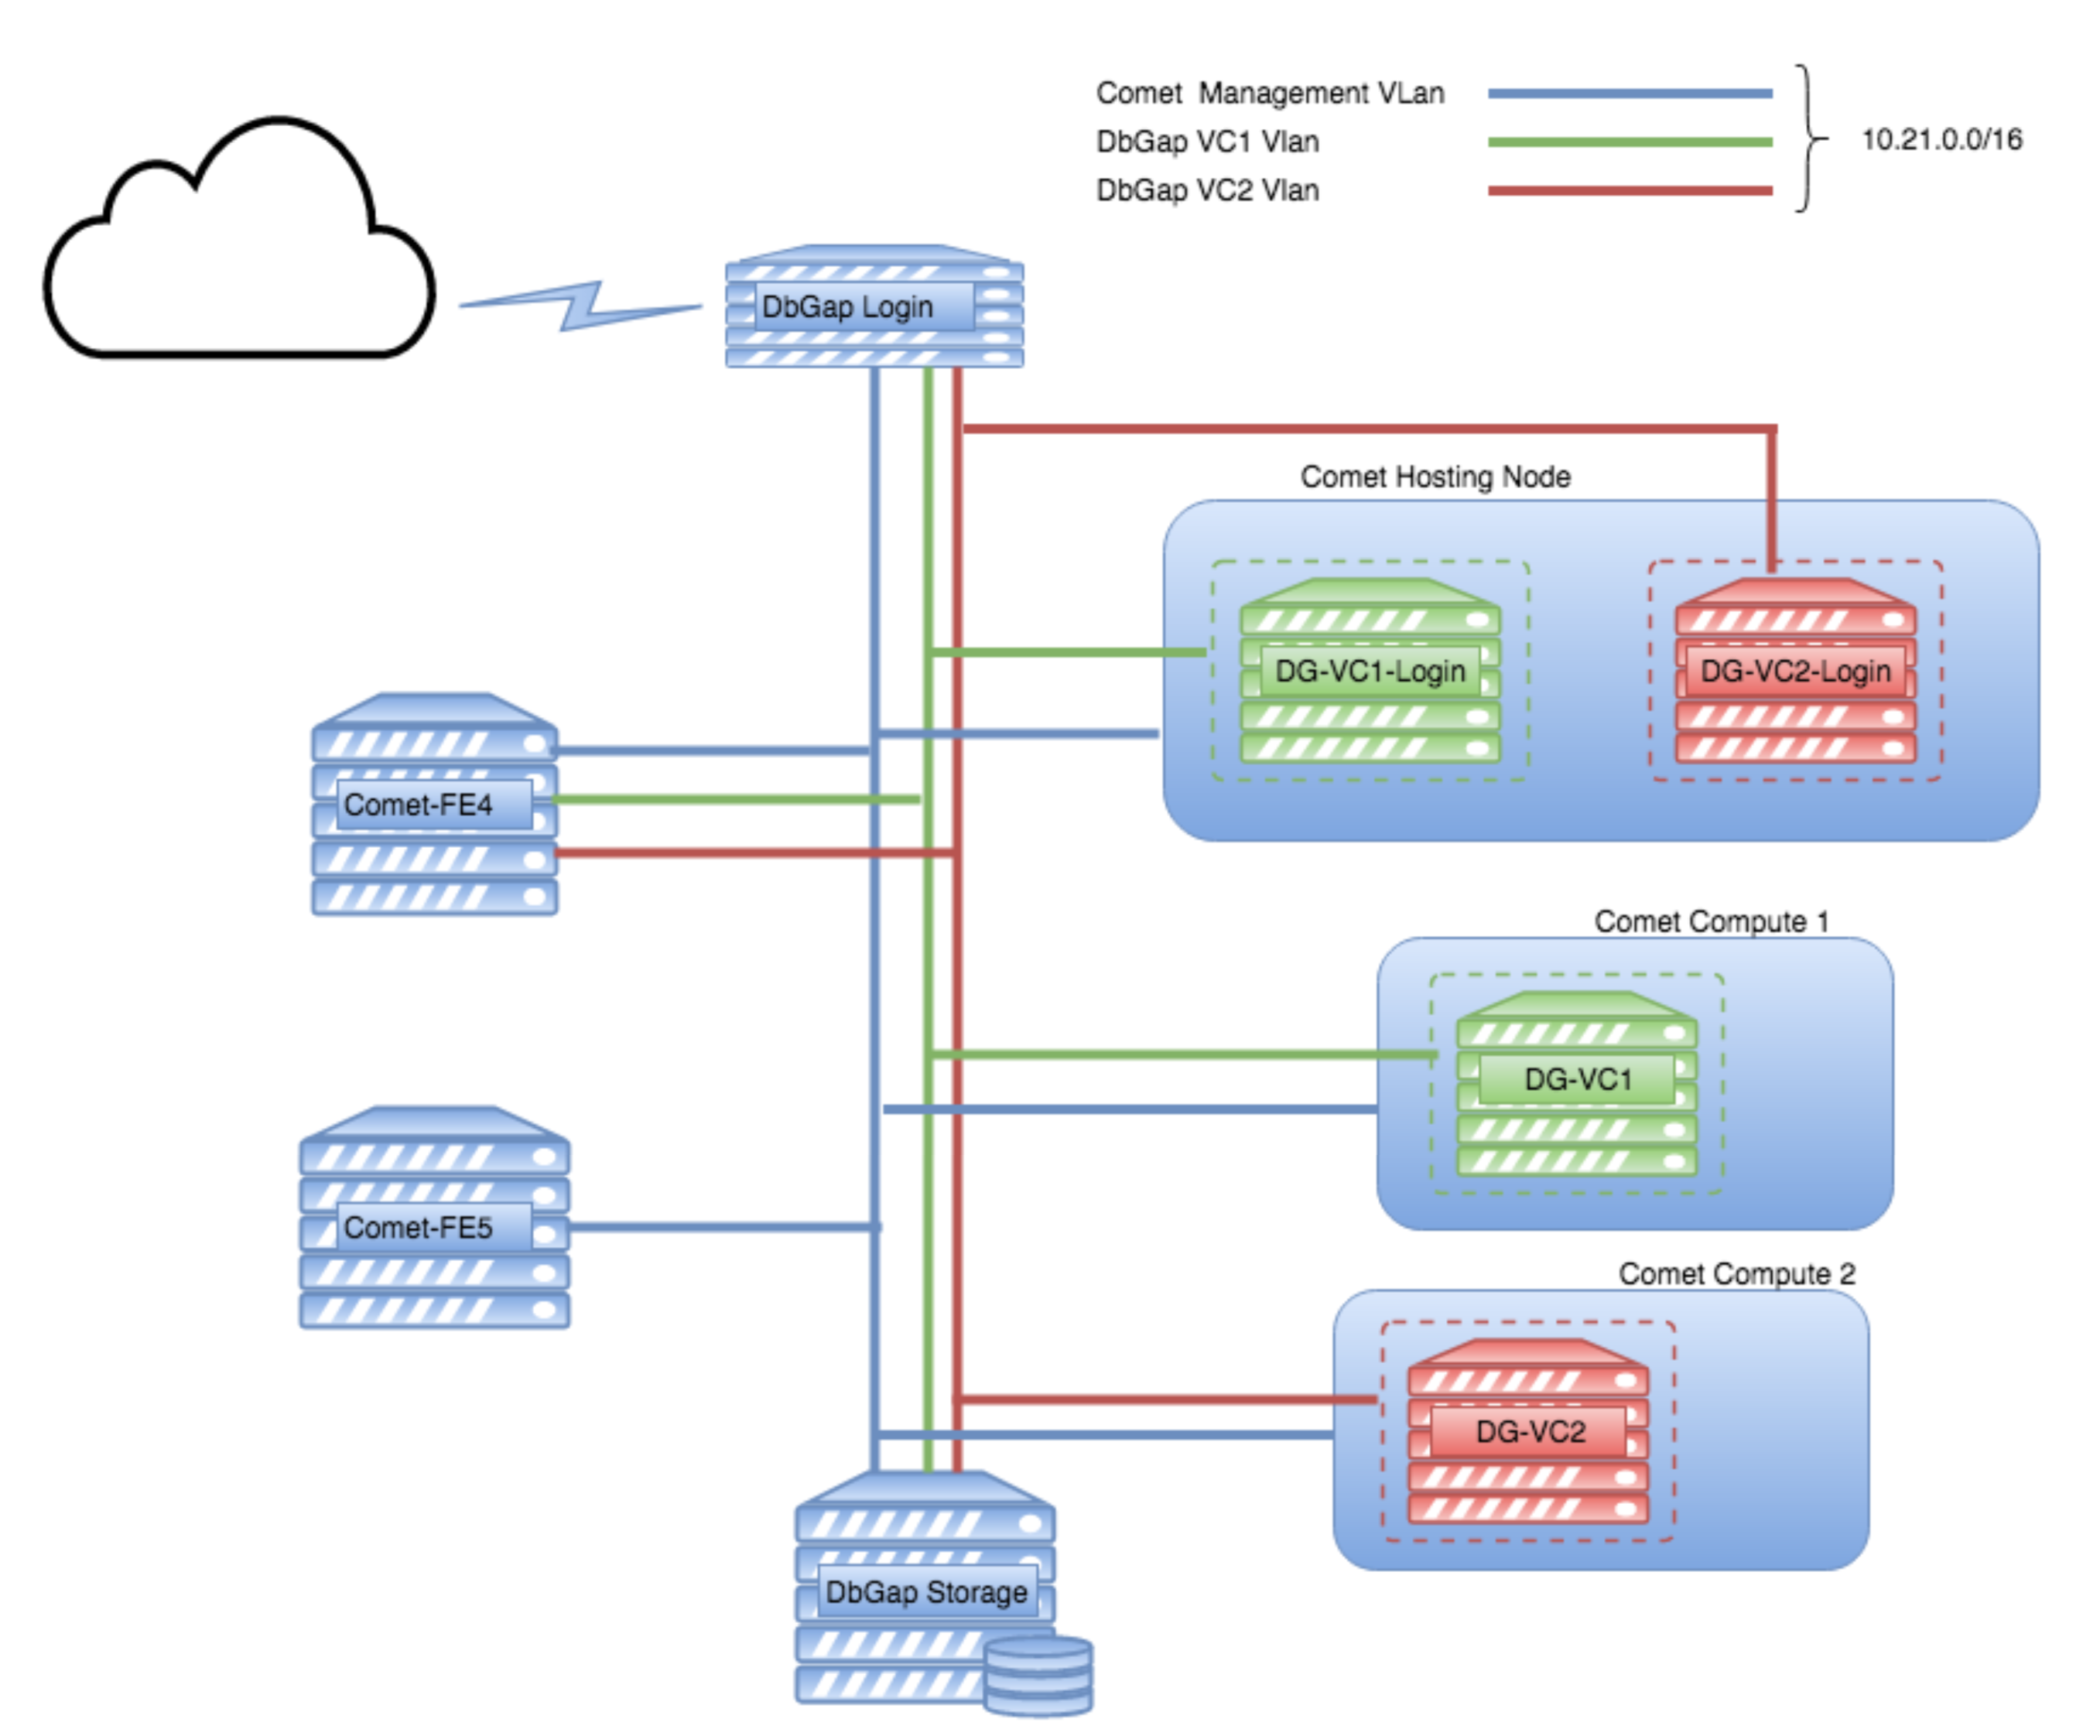
\includegraphics[width=\linewidth]{images/dbgap.png}
  \caption{DBGAP Comet Architecture.}\label{fig:car}
  \Description{The DBGAP comet architecture.}
\end{figure}


\TODO{This is just copied and needs to be organizes and only relavant portions need to be explained}


Below is a list of questions to be addressed as a result of this 
requirements document:

Question
Plan

Implementation Details
How are nodes provisioned?
Both login and compute nodes will be cloned from a master
reference image that is created and maintained by the Systems Group.
How are nodes configured for network?
Via dhcp from comet-fe4
IB interface needs to be configured as well.
Does this get done via DHCP has well?
      How do we get configuration data such as user, group, slurm config
and other such info onto the nodes.
 Using Rocks and custom CM from Comet's Management node (Comet-fe4). Although every
DbGap cluster will have its own Vlan they will all share the Comet management IP space.
Comet-fe4 will bridge the Vlans allowing it to act as the mangement node for all DbGap clusters.
Don't have to mantain seperate frontends for every cluster.
Allows us to use a single image for both compute and login nodes.
Smaller non-persistant image.
       Need to either create custom passwd,shadow, and group files
for each Cluster or just create customized access.conf file for
cluster's login node.
Need to set host name. Using dhcp to does this will require a
modificatio of Rocks.
Slurm config and mount points will be part of CM scripts.
  Will compute node images be persistent?
 No, node images will not be synced to the image server so any changes
made to the node during a job will be discarded. This means that all user
data will need to be copied off once the jobs completes.
  Nodes should be set not to since back.
 Will login nodes be persistent.
  Undeterminded. If we can use an NFS mount to save slurm state then there is
no need for the login nodes to be persistent either.
      How are nodes patched and upgraded?
Only the reference image needs to be maintained. Since nodes are not persistent the
node will get a fresh clone of the reference image with the latest updates every time it
boots.
   Should have scrips that automate the recreation of the
clones. Needs to be able to handle insuring running nodes
get the new image the next time they run.
 How will users submit jobs.
  DbGap VC users will simply submit jobs to a local slurm server. The slurm sever wil have
hooks that will utilize cloudmesh to transparently start a Comet VC job.
      Can DbGap cluster users access lustre.
Yes. Using bind mounts DbGap VCs could have access to a restricted subdirectory
which contains only their group's DbGap data.
   DbGap compute nodes will need interfaces and IPs on
the lustre Pkey. (Need to check that we have the IP
space)
 How will data be moved in and out of the DbGap clusters
  ??
    Will every job run on a dedicated node or do we allow node sharing.
Undetermined. We could allow multiple jobs within the DbGap VC to run on the same
node. This could be benificial for the users because it would be cheeper to run smaller
jobs. However, this could make maintainice more labor intensive since Systems group
admins would need to intervene to insure nodes rebooted to get updates.



\subsection{Features}

cfengine

uses slurm via virtual machine management

uses Infiniband

uses lustre

restricted lustre directory for dbGap user group directory.

Auto home for users in dbGap group.

Nucleus REST API


\section{dbgap 2}

\hypertarget{dbgap-virtual-cluster-plan}{%
\section{dbGaP Virtual Cluster Plan}\label{dbgap-virtual-cluster-plan}}


\subsection{Goals}

\begin{itemize}
\item
  Provide a workable Virtual Cluster template that meets the
  requirements for users processing DbGap data.
\end{itemize}

\hypertarget{background-and-strategic-fit}{%
\subsection{Background and strategic
fit}\label{background-and-strategic-fit}}

\hypertarget{assumptions}{%
\subsection{Assumptions}\label{assumptions}}

\begin{itemize}
\item
  Every Project/Group using DbGap will have it's own Virtual Cluster
  (VC).
\item
  The HPC Systems group will manage the dbGaP VCs.
\item
  dbGaP VCs will comply with dbGaP guidelines.
  (\url{https://osp.od.nih.gov/wp-content/uploads/NIH_Best_Practices_for_Controlled-Access_Data_Subject_to_the_NIH_GDS_Policy.pdf})
\end{itemize}



\hypertarget{questions}{%
\subsection{Questions}\label{questions}}

Below is a list of questions to be addressed as a result of this
requirements document:

\begin{table*}
\begin{tabular}{|p{4cm}|p{4cm}|p{4cm}|}
\toprule
\textbf{Question} & \textbf{Plan} & \textbf{Implimentation
Details}\\
\midrule

How are nodes provisioned?
 & 
Both login and compute nodes will be cloned from a master
reference image that is created and maintained by the Systems
Group.
 & 
~
\\
How are nodes configured for network?
 & 
Via dhcp from comet-fe4
 & 
IB interface needs to be configured as well.
Does this get done via DHCP has well?
\\

How do we get configuration data such as user, group, slurm config

and other such info onto the nodes.
 & 
Using Rocks and custom CM from Comet's Management node (Comet-fe4).
Although every
DbGap cluster will have its own Vlan they will all share the Comet
management IP space.
Comet-fe4 will bridge the Vlans allowing it to act as the mangement node for all DbGap clusters.

\begin{itemize}
\item
  Don't have to mantain seperate frontends for every cluster.
\item
  Allows us to use a single image for both compute and login nodes.
\item
  Smaller non-persistant image.
\end{itemize}
 & 
Need to either create custom passwd,shadow, and group files
for each Cluster or just create customized access.conf file for
cluster's login node.

Need to set host name. Using dhcp to does this will require a
modificatio of Rocks.
Slurm config and mount points will be part of CM scripts.
\\

Will compute node images be persistent?
 & 
No, node images will not be synced to the image server so any changes
made to the node during a job will be discarded. This means that all
user
data will need to be copied off once the jobs completes.
 & 
Nodes should be set not to since back.
\\

Will login nodes be persistent.
& 
Undeterminded. If we can use an NFS mount to save slurm state then there
is no need for the login nodes to be persistent either.
& 
~
\\

How are nodes patched and upgraded?
 & 
Only the reference image needs to be maintained. Since nodes are not
persistent the
node will get a fresh clone of the reference image with the latest
updates every time it
boots.
 & 
Should have scrips that automate the recreation of the
clones. Needs to be able to handle insuring running nodes
get the new image the next time they run.
\\

How will users submit jobs.
 & 
DbGap VC users will simply submit jobs to a local slurm server. The
slurm sever will have
hooks that will utilize cloudmesh to transparently start a Comet VC
job.
 & 
~
\\

Can DbGap cluster users access lustre.
 & 
Yes. Using bind mounts DbGap VCs could have access to a restricted
sub-directory
which contains only their group's DbGap data.
 & 
DbGap compute nodes will need interfaces and IPs on
the lustre Pkey. (Need to check that we have the IP
space)
\\
How will data be moved in and out of the DbGap clusters & ?? &
~\\

Will every job run on a dedicated node or do we allow node
sharing.
 & 
Undetermined. We could allow multiple jobs within the DbGap VC to run on
the same
node. This could be beneficial for the users because it would be cheaper to run smaller
jobs. However, this could make maintainance more labor intensive since
Systems group

admins would need to intervene to insure nodes rebooted to get
updates. & ~ 
\\
\bottomrule
\end{tabular}
\end{table*}

\subsection{To Do.}

\begin{itemize}
\item
  Get dhcp of dbGap nodes working.
\item
  Configuration management~

  \begin{itemize}
  \item
    get cfengine on front end. (trevor)
  \item
    slurm client/server - (slurm cluster named after frontend name)
  \item
    IPs for IB interfaces -should come from rocks database perhaps using
    Scotts Rocks 7 cfengine plugin.
  \item
    Create bind mount of Lustre from restricted lustre directory for
    dbGap user group directory.
  \item
    Auto home for users in dbGap group.
  \end{itemize}
\item
  Things that don't come from cfengine

  \begin{itemize}
  \item
    Nucleus API key
  \item
    Mysql password for Slurm.
  \item
    Shadow File
  \item
    SSH host keys for host based management.
  \end{itemize}
\end{itemize}


\section{OTHER}

Example Figure \ref{fig:car}.

Example citation \cite{comet17tails}.
